% -*- mode: latex; coding: latin-1-unix -*- %

\section{Analyse Statique} 

Nous avons dans cette partie repr�sent� des fonctions cl�s de notre
programme � l'aide de CFA. Ceux-ci nous servent � effectuer une
s�rie de tests statiques des fonctions critiques du puissance4. Nous
trouverons dans l'ordre la fonction principale de notre moteur de jeu,
puis dans une seconde partie les CFA repr�sentant la partie IA du programme. 

Pour plus de clart� les deux CFA principaux que sont \texttt{start} et
\texttt{IA} sont amput�s des fonctions auquel ils font appel. On consid�rera d�s
lors que ces appels effectuent la fonctions pour lesquel ils sont
�crits et ne provoquent pas de bug du programme. Ces fonctions sont
repr�sent�es par la suite et sont analys�es s�par�ment. 
\subsection{GameEngine}

\begin{figure}[h]
\begin{center}
  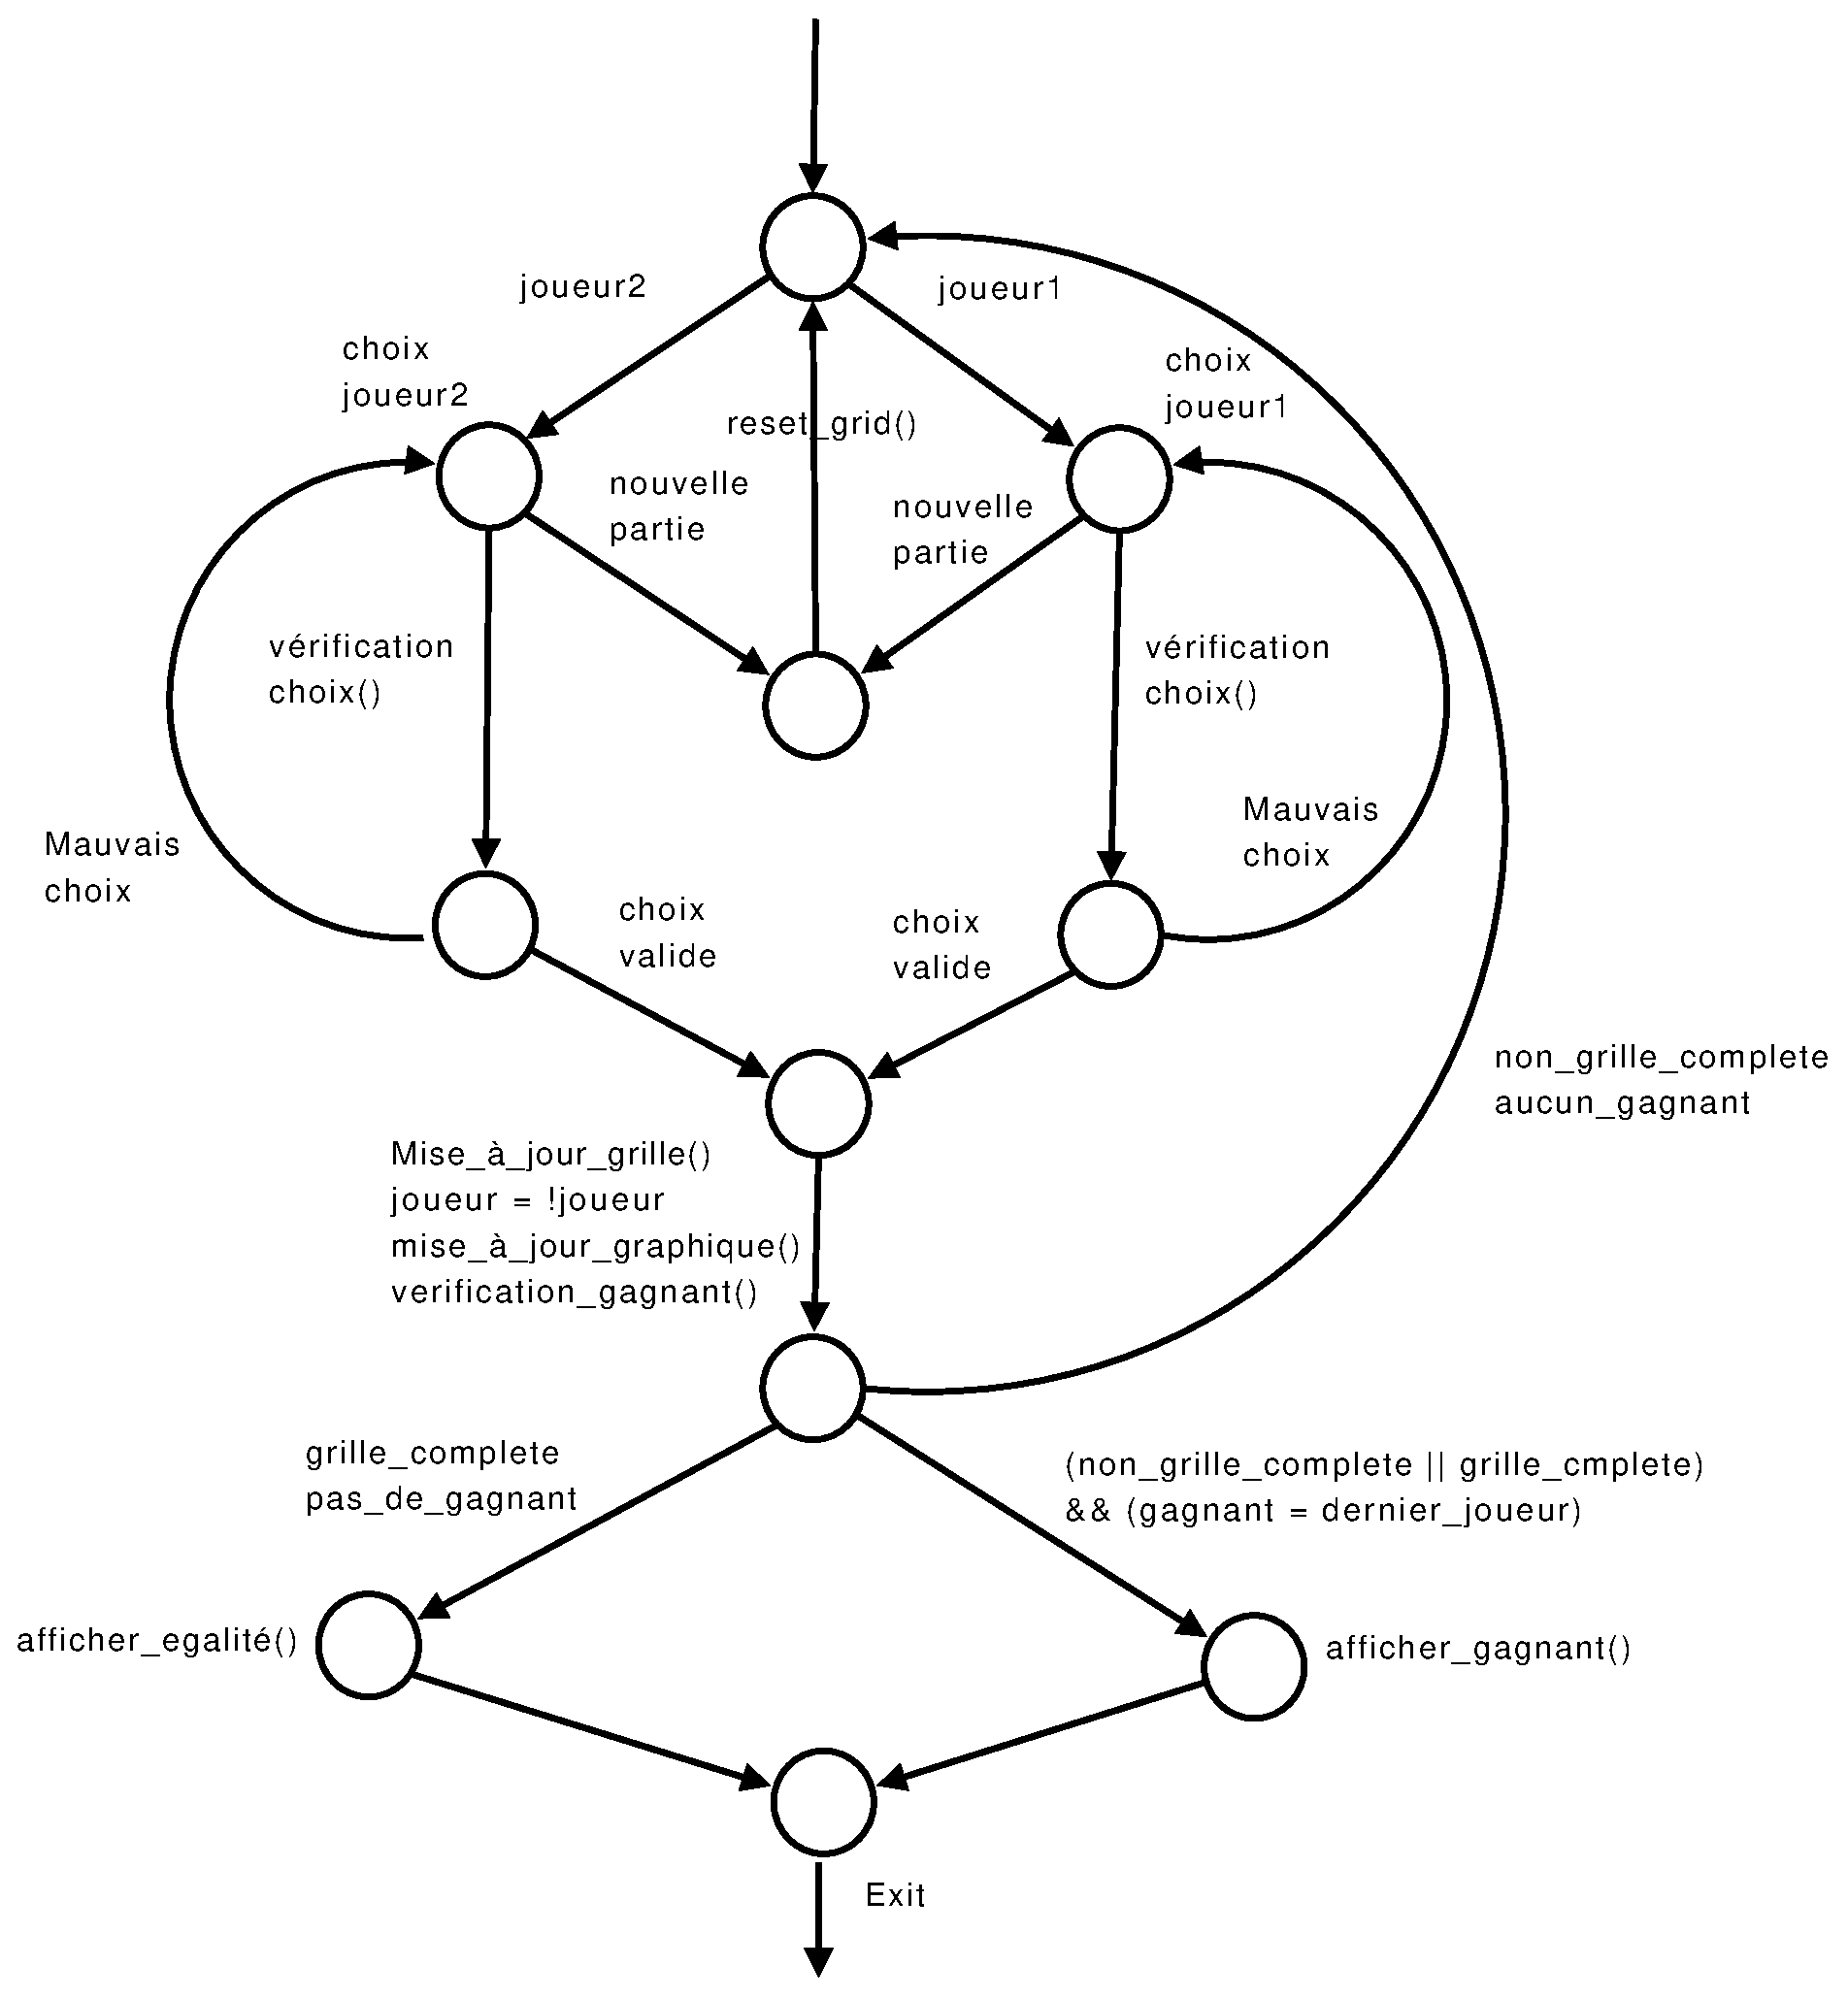
\includegraphics[scale=0.6]{start}
  \caption{Fonction start}
\end{center}
\end{figure}

\newpage
DT1=\{joueur1,joueur2,0=<choixJoueur1=<6,0=<choixJoueur2=<6,grille\_vide\}
En supposant qu'aucun des deux joueurs ne r�initialise la partie, et
que celle-ci ce termine, nous obtenons deux chemins possible :\\
\{0-2-5-6-7-0-3-4-6-7-...-9-10\} // partie avec un gagnant \\
\{0-2-5-6-7-0-3-4-6-7-...-8-10\} // partie avec un match nul\\

En prenant comme crit�re de couverture l'ensemble de tous les noeuds
nous obtenons un TER 1 = 9/11 = 81\%.\\

DT2=\{joueur1,joueur2,choixJoueur1,0=<choixJoueur2=<6,grille\_vide\}

\subsubsection{Les fonctions}
\texttt{v�rification\_choix()}\\
\begin{figure}[h]
\begin{center}
  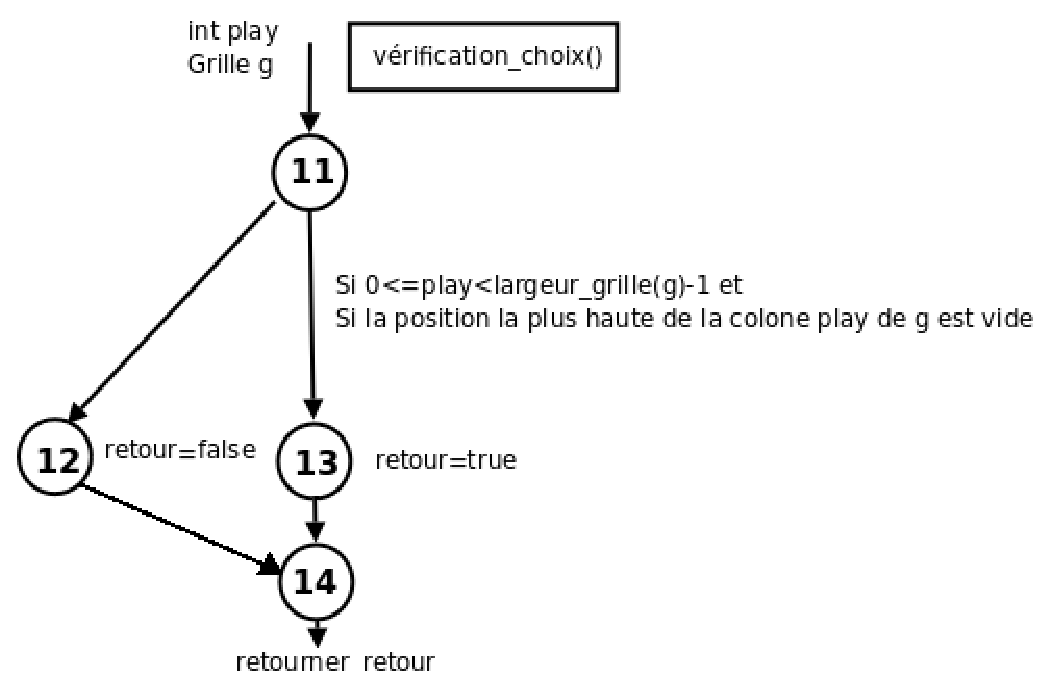
\includegraphics[scale=0.6]{verification_choix}
  \caption{Fonction v�rification choix}
\end{center}
\end{figure}

\newpage
\texttt{v�rification\_gagnant()}\\
\begin{figure}[h]
\begin{center}
  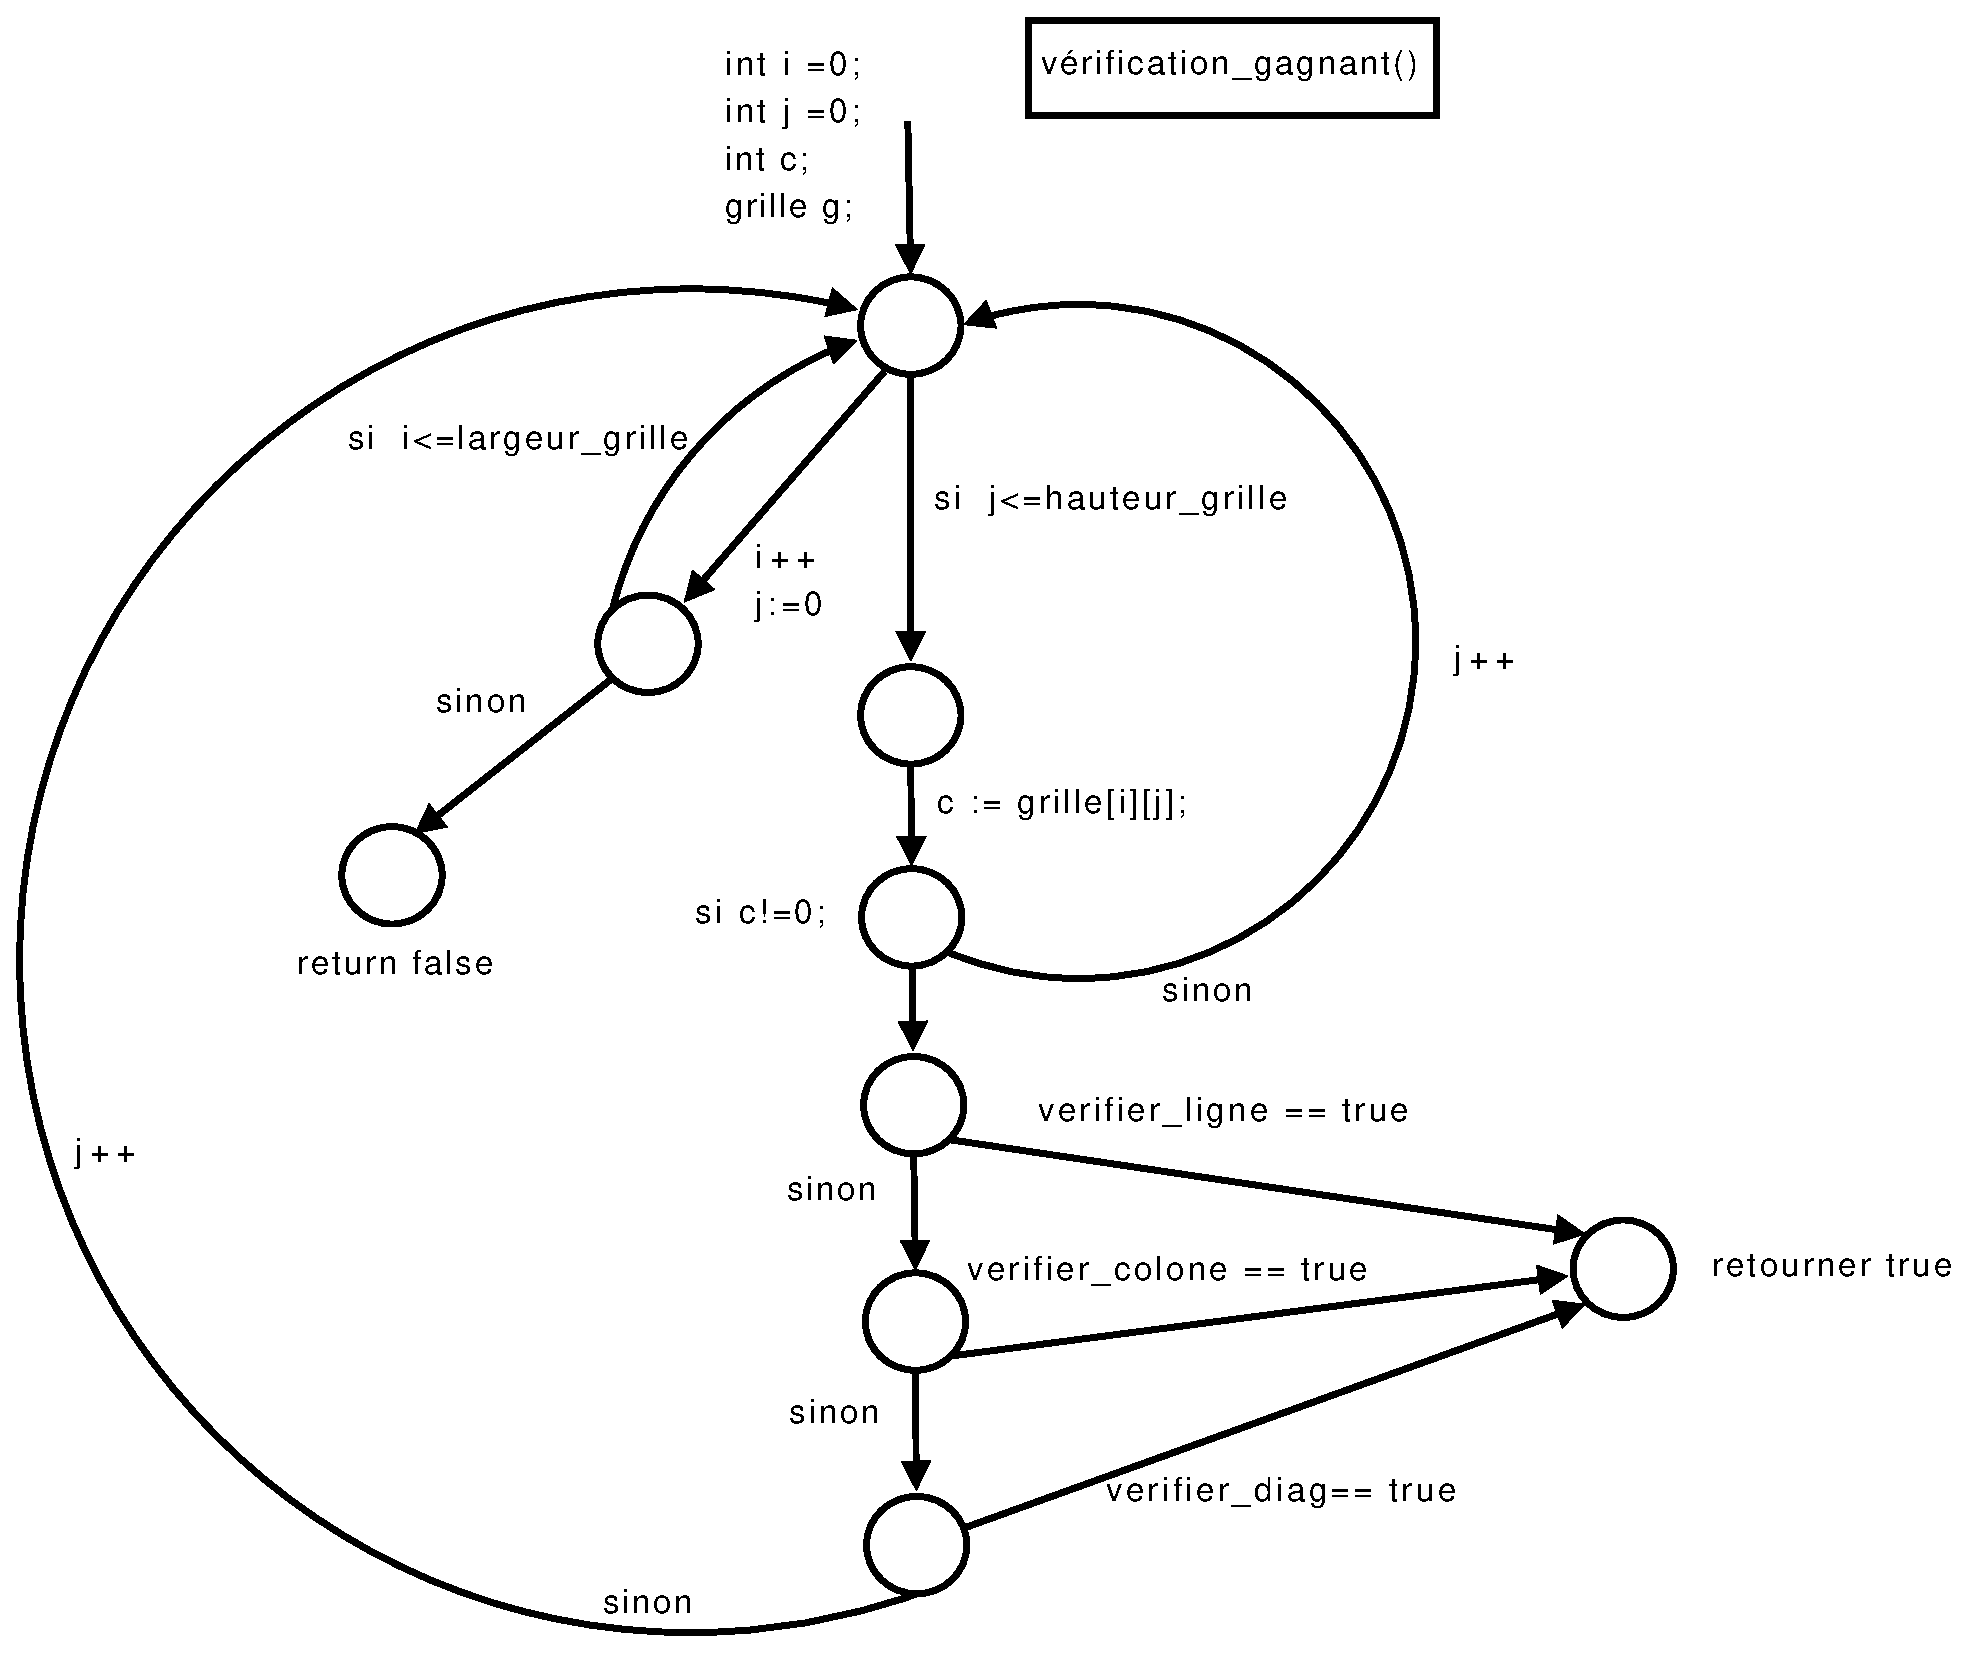
\includegraphics[scale=0.6]{verification_gagnant}
  \caption{Fonction v�rification gagnant}
\end{center}
\end{figure}

\newpage
\subsection{IA}

\begin{figure}[h]
\begin{center}
  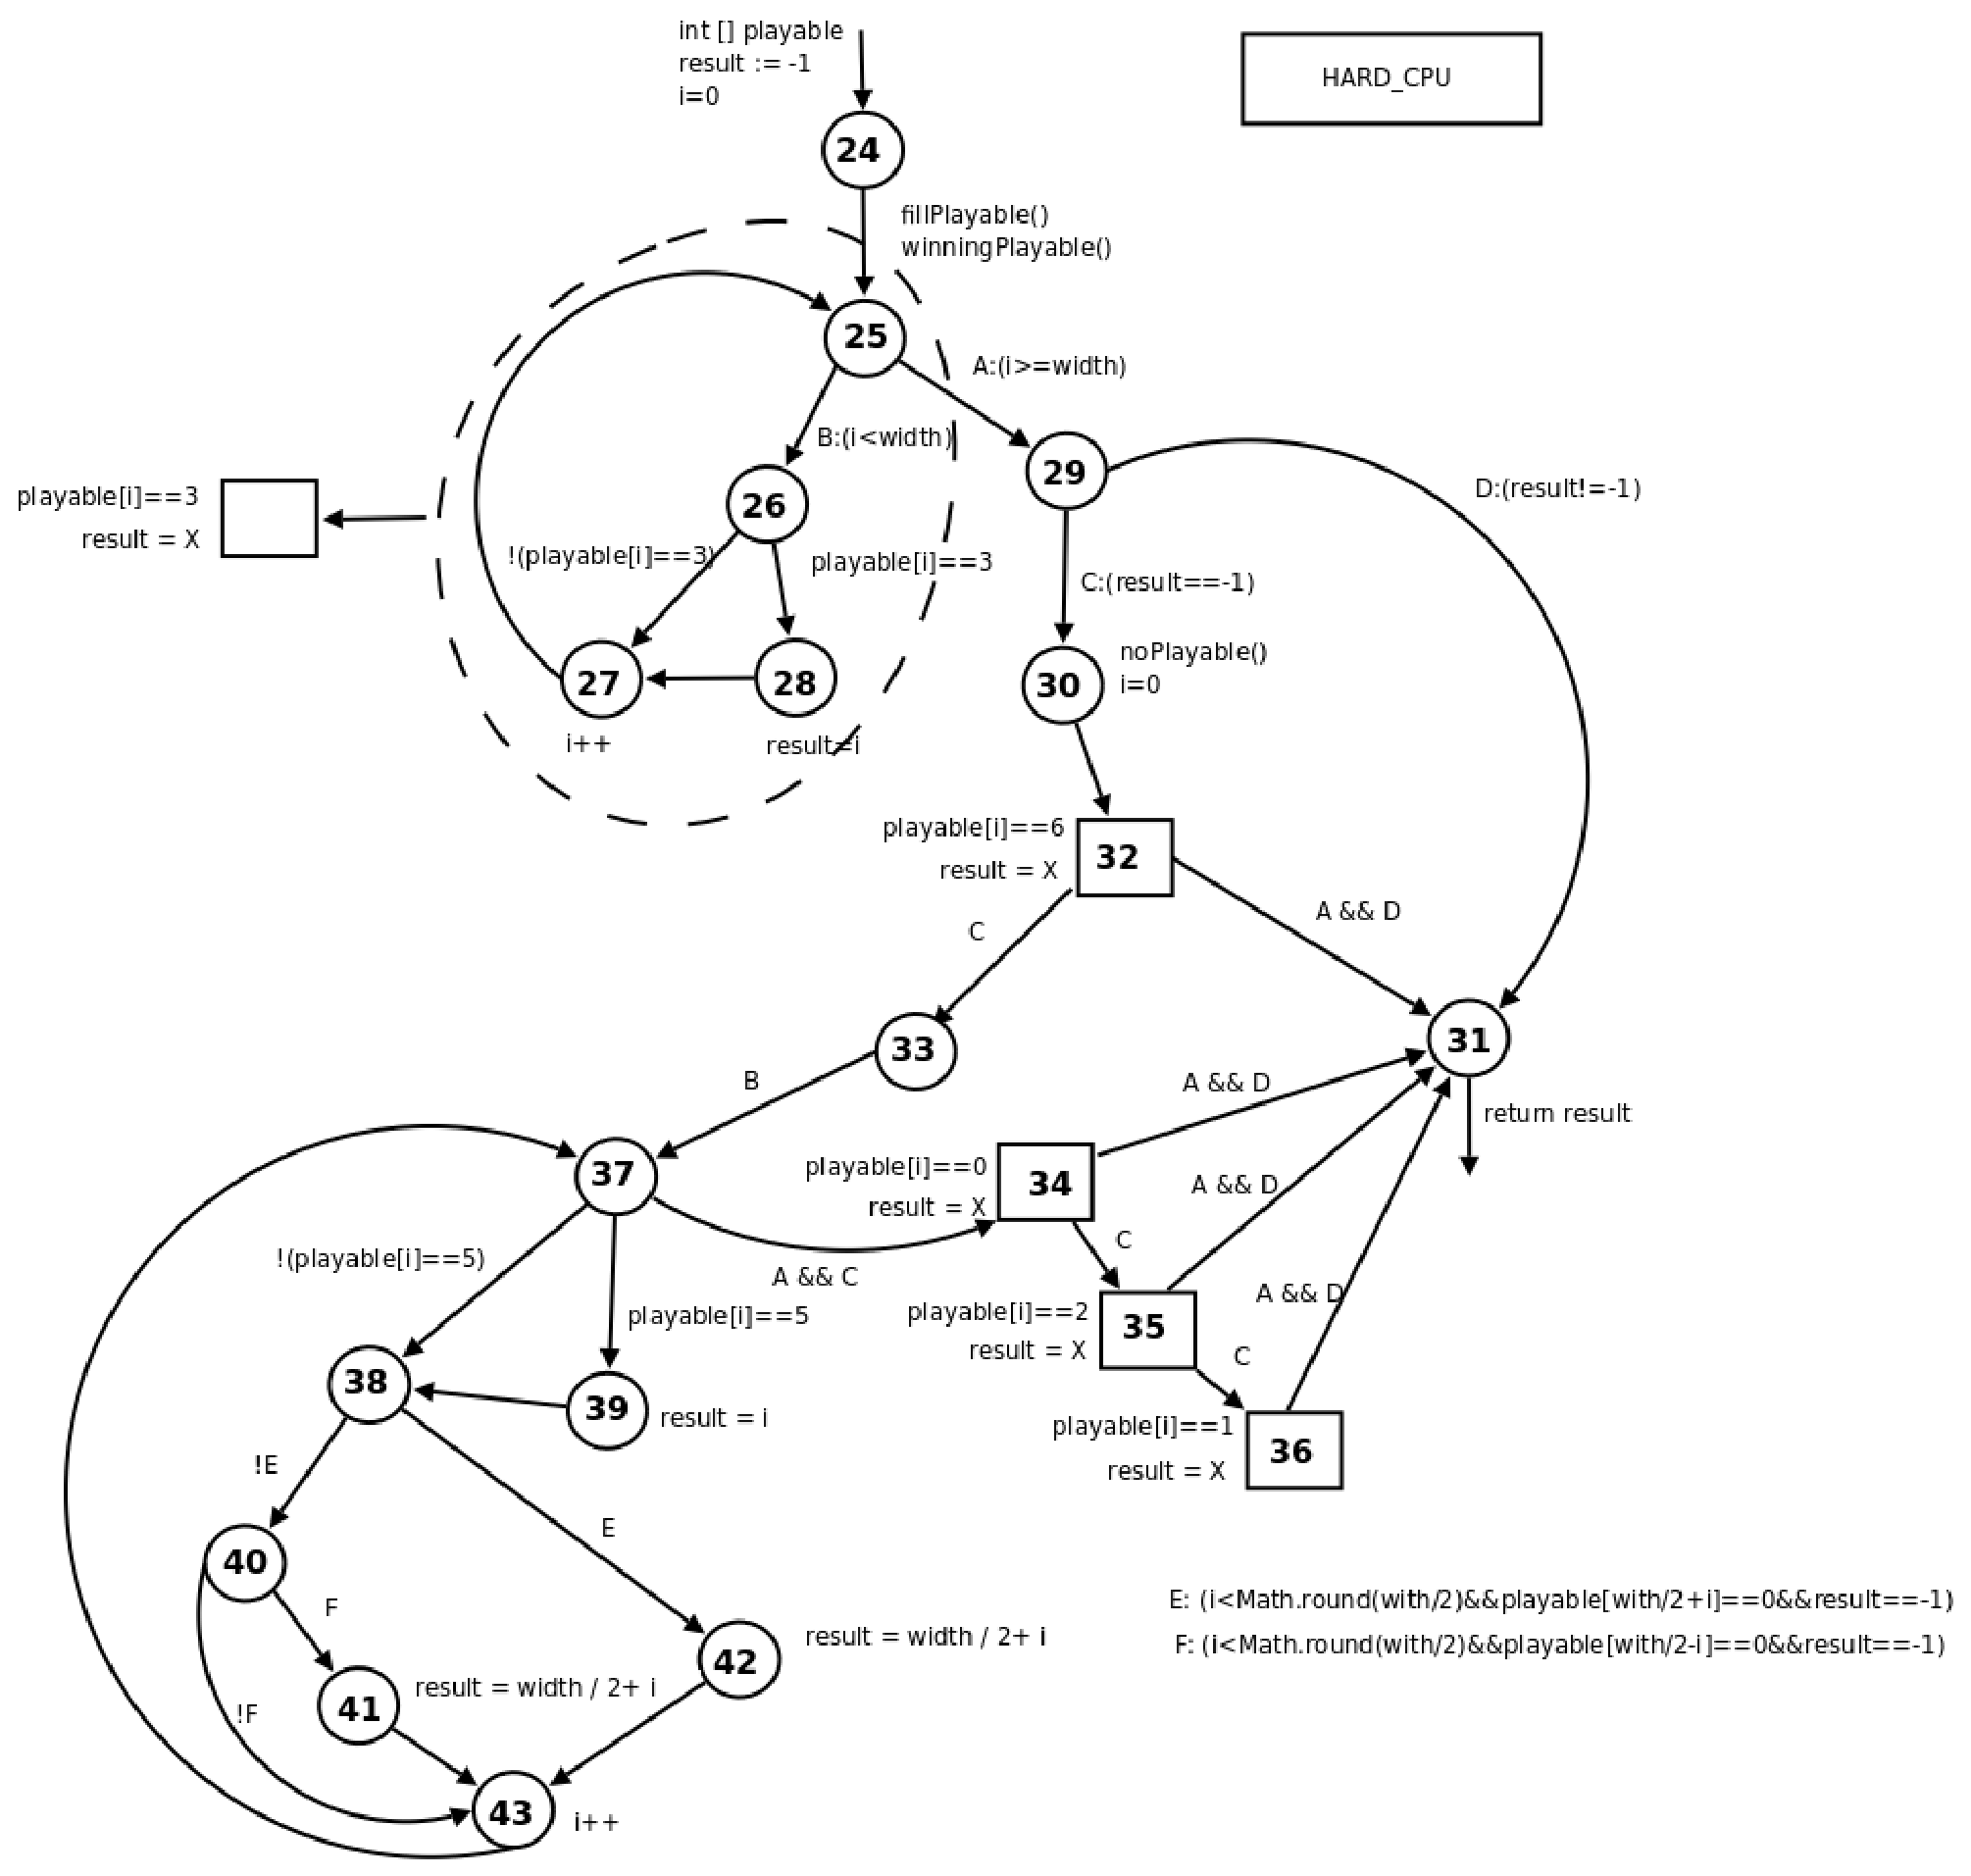
\includegraphics[scale=0.5]{IA}
  \caption{IA du programme}
\end{center}
\end{figure}


\newpage
\subsubsection{Les fonctions}
\texttt{fillPlayable()}\\
\begin{figure}[h]
\begin{center}
  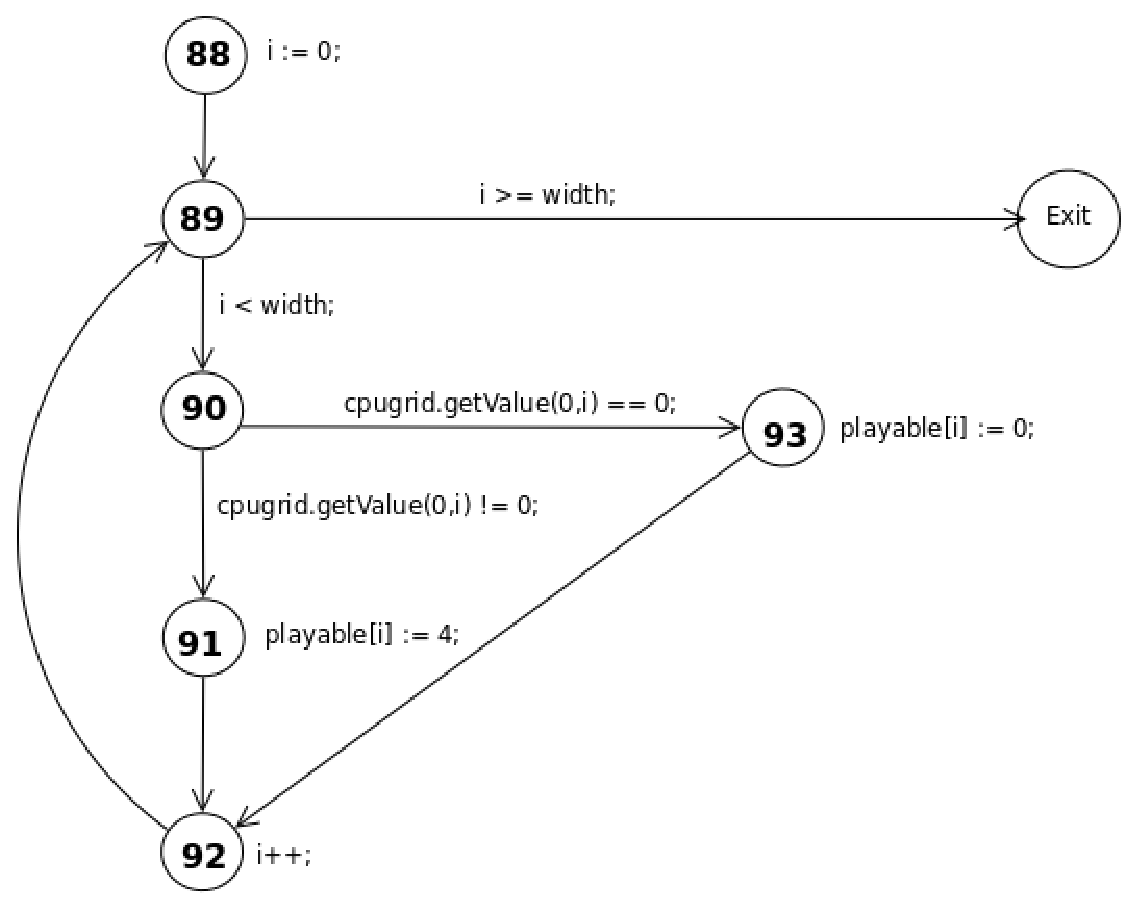
\includegraphics[scale=0.6]{fillPlayable}
  \caption{Fonction fillPlayable}
\end{center}
\end{figure}

\newpage
\texttt{winningPlayable()}\\
\begin{figure}[h]
\begin{center}
  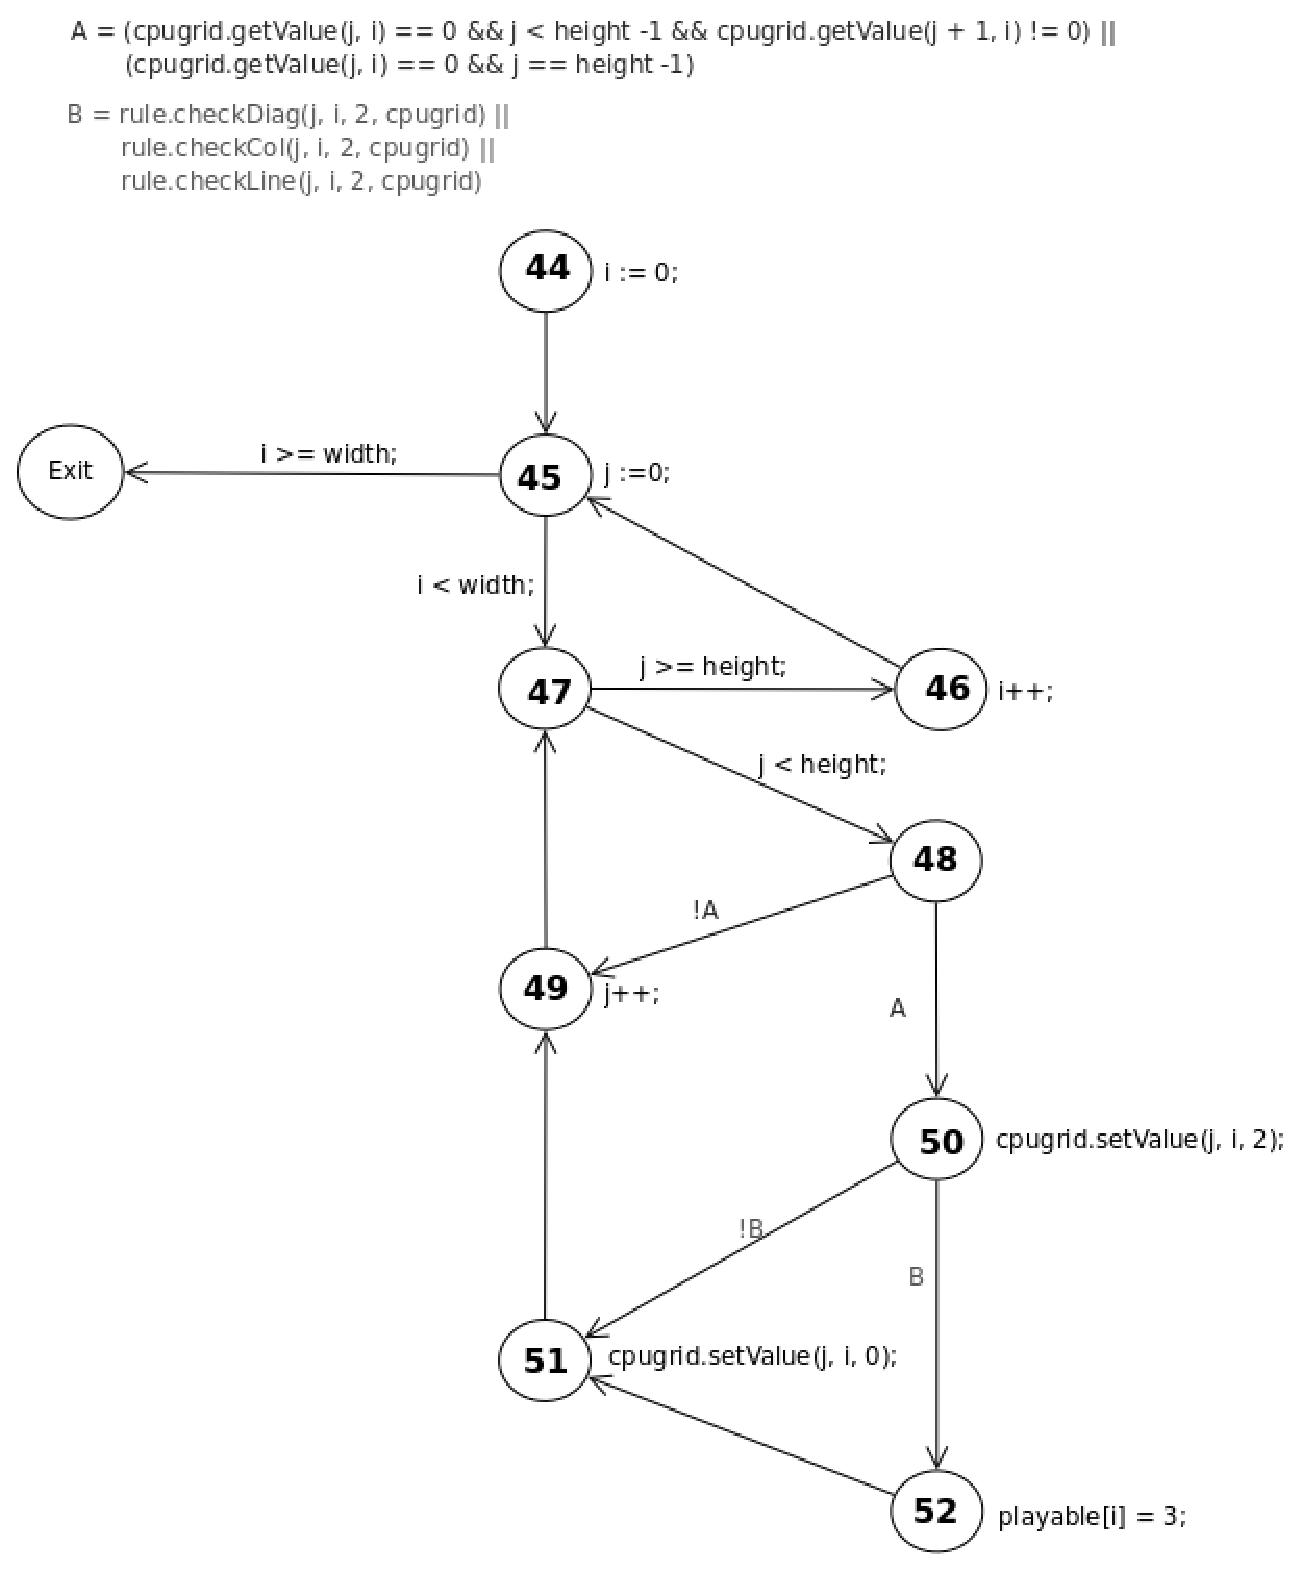
\includegraphics[scale=0.6]{winningPlayable}
  \caption{Fonction winningPlayable}
\end{center}
\end{figure}

\newpage
\texttt{noPlaybale()}\\
\begin{figure}[h]
\begin{center}
  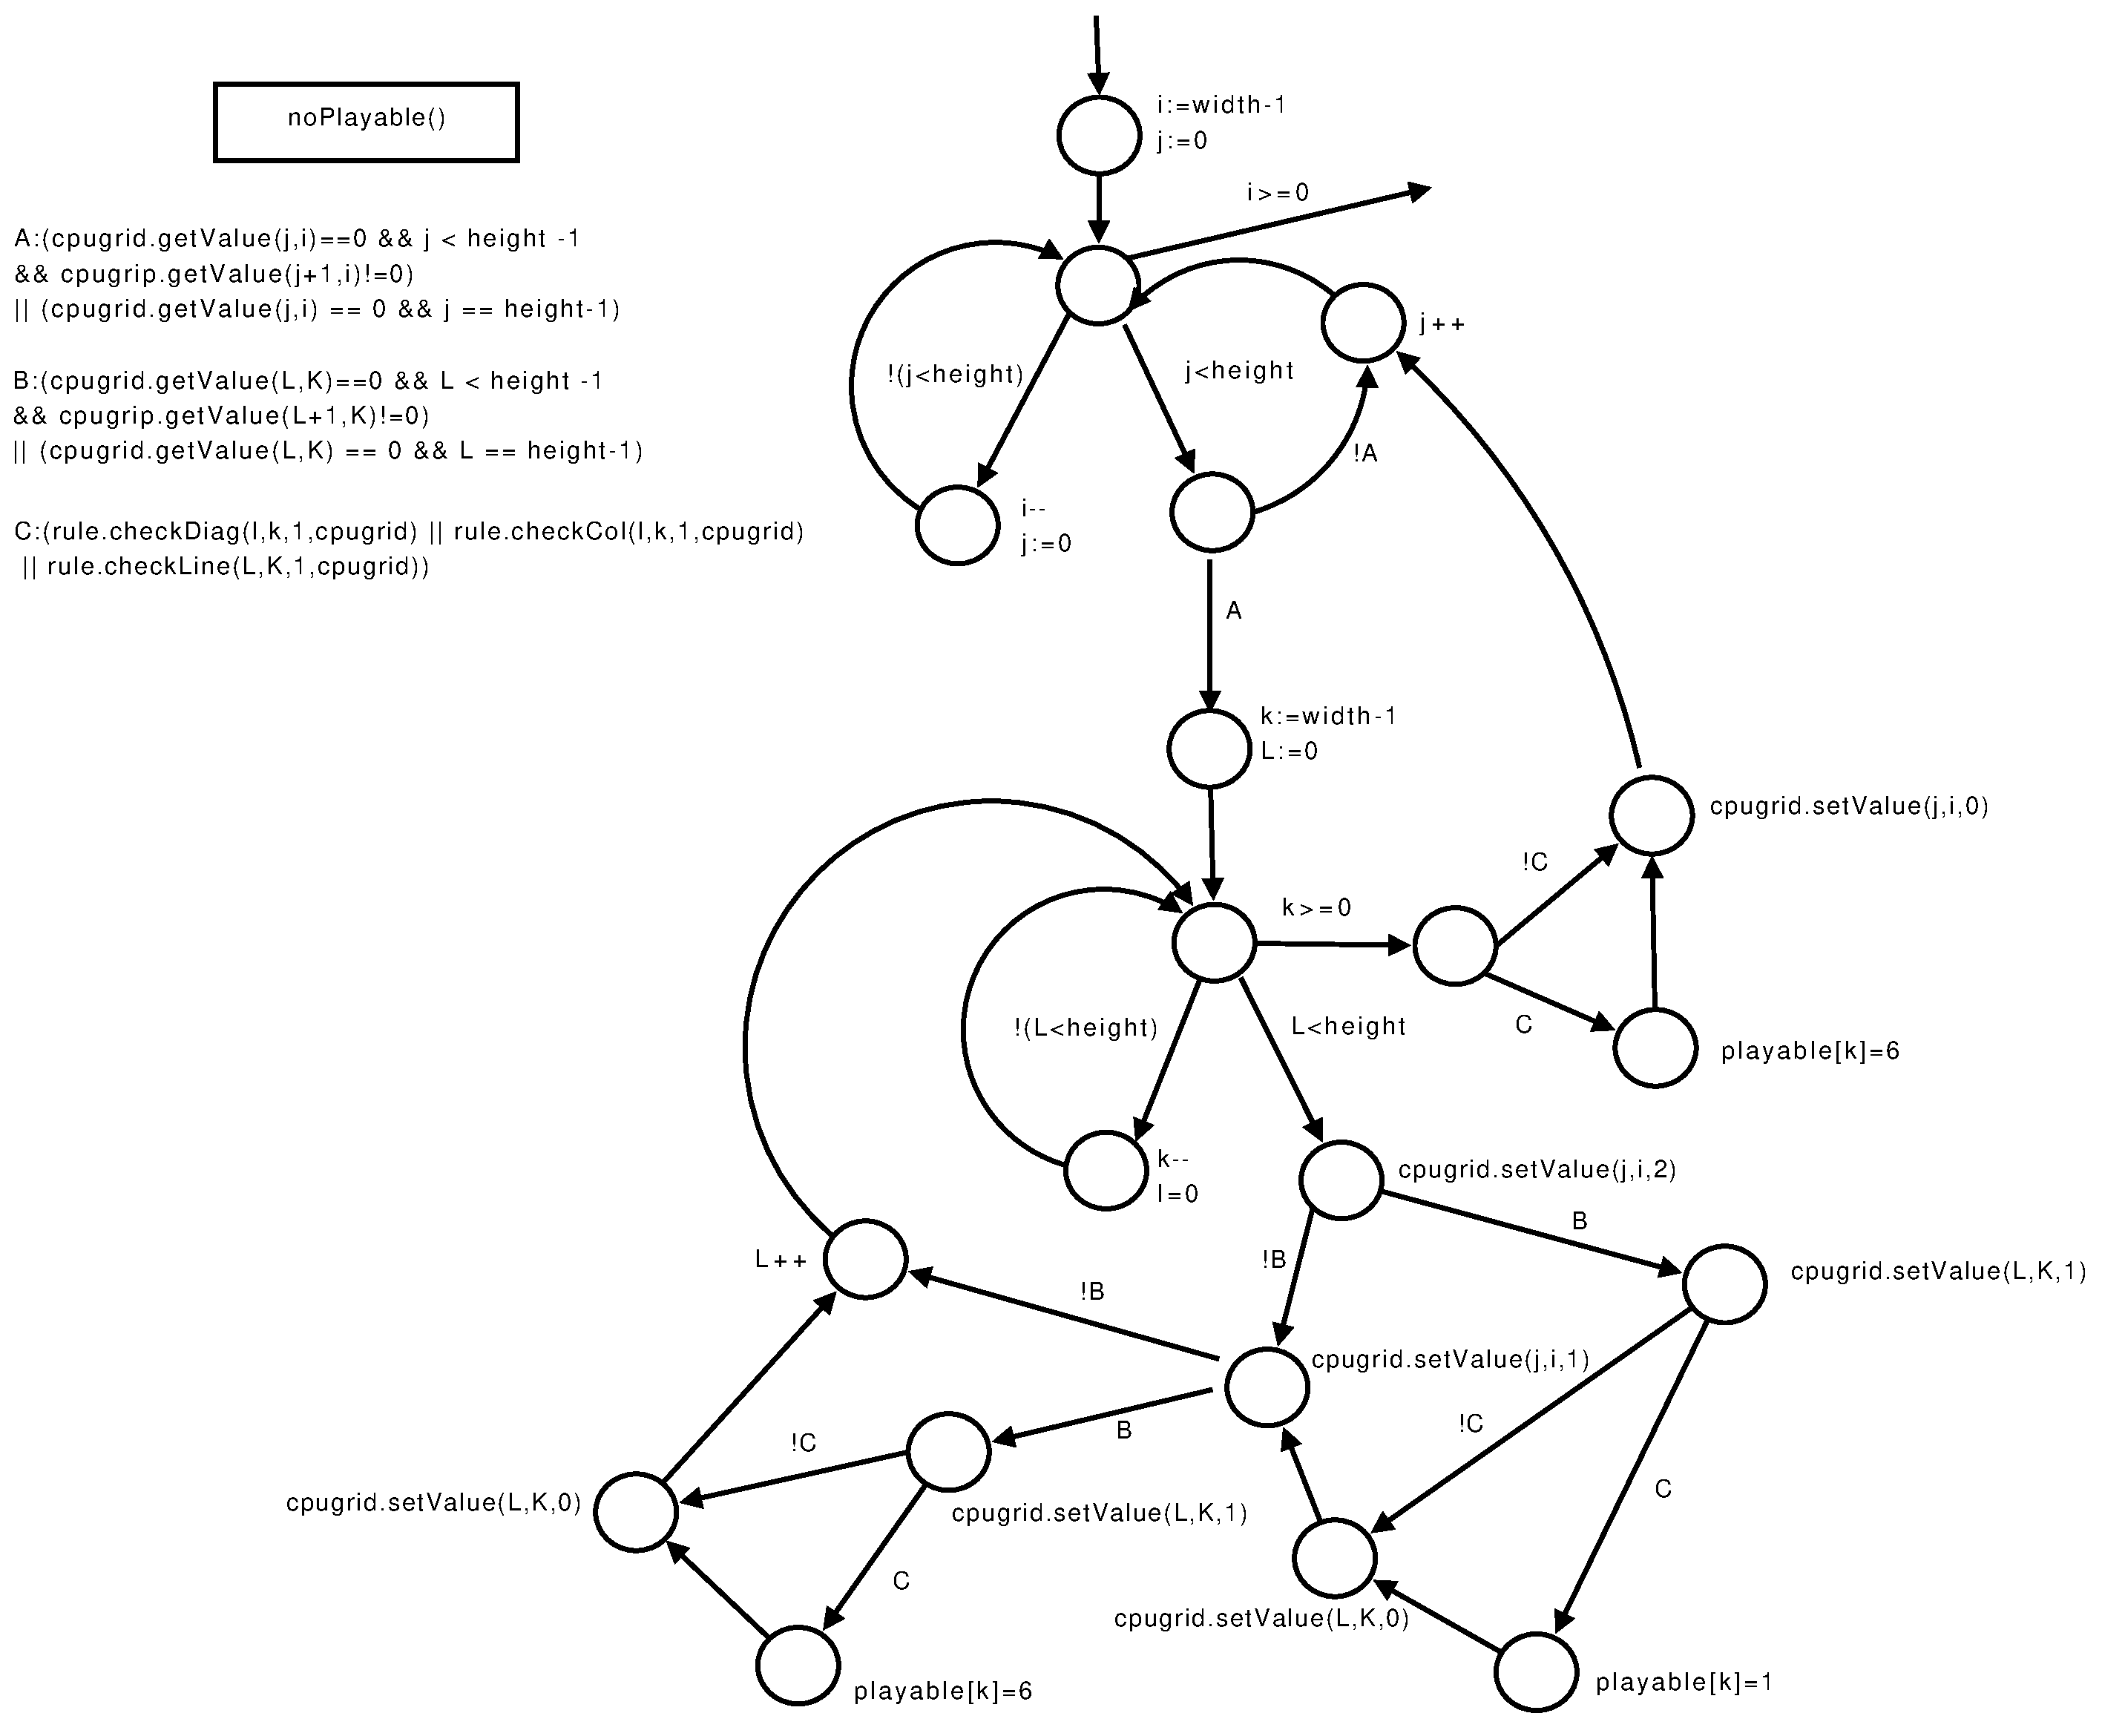
\includegraphics[scale=0.5]{noplayable}
  \caption{Fonction noPlayable}
\end{center}
\end{figure}

\newpage
\texttt{breakStrategy()}\\
\begin{figure}[h]
\begin{center}
  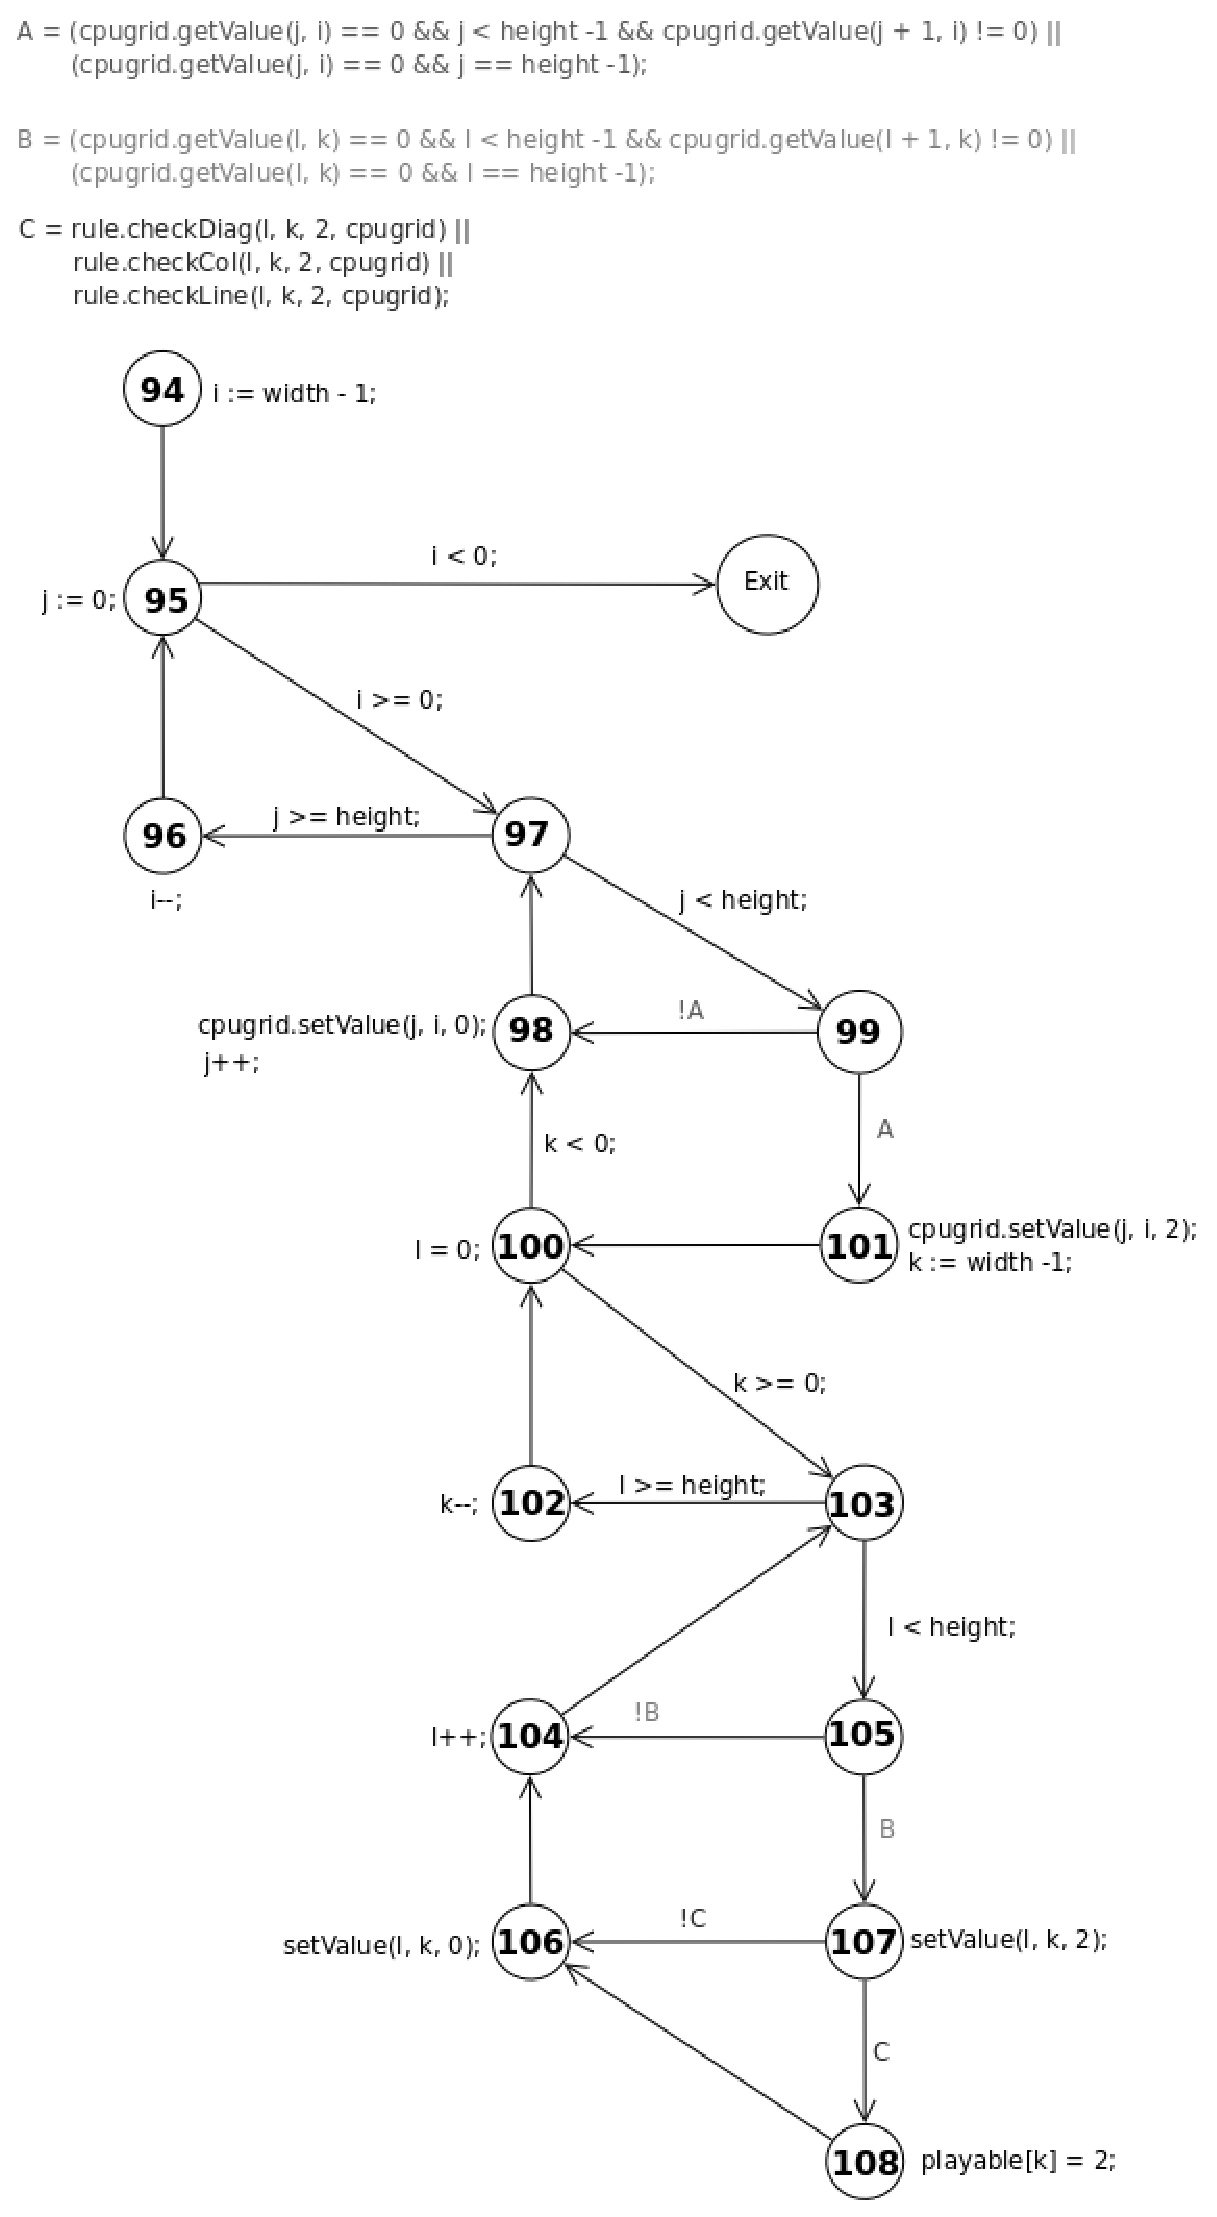
\includegraphics[scale=0.4]{breakStrategy}
  \caption{Fonction breakStrategy}
\end{center}
\end{figure}

\newpage
\texttt{strategy()}\\
\begin{figure}[h]
\begin{center}
  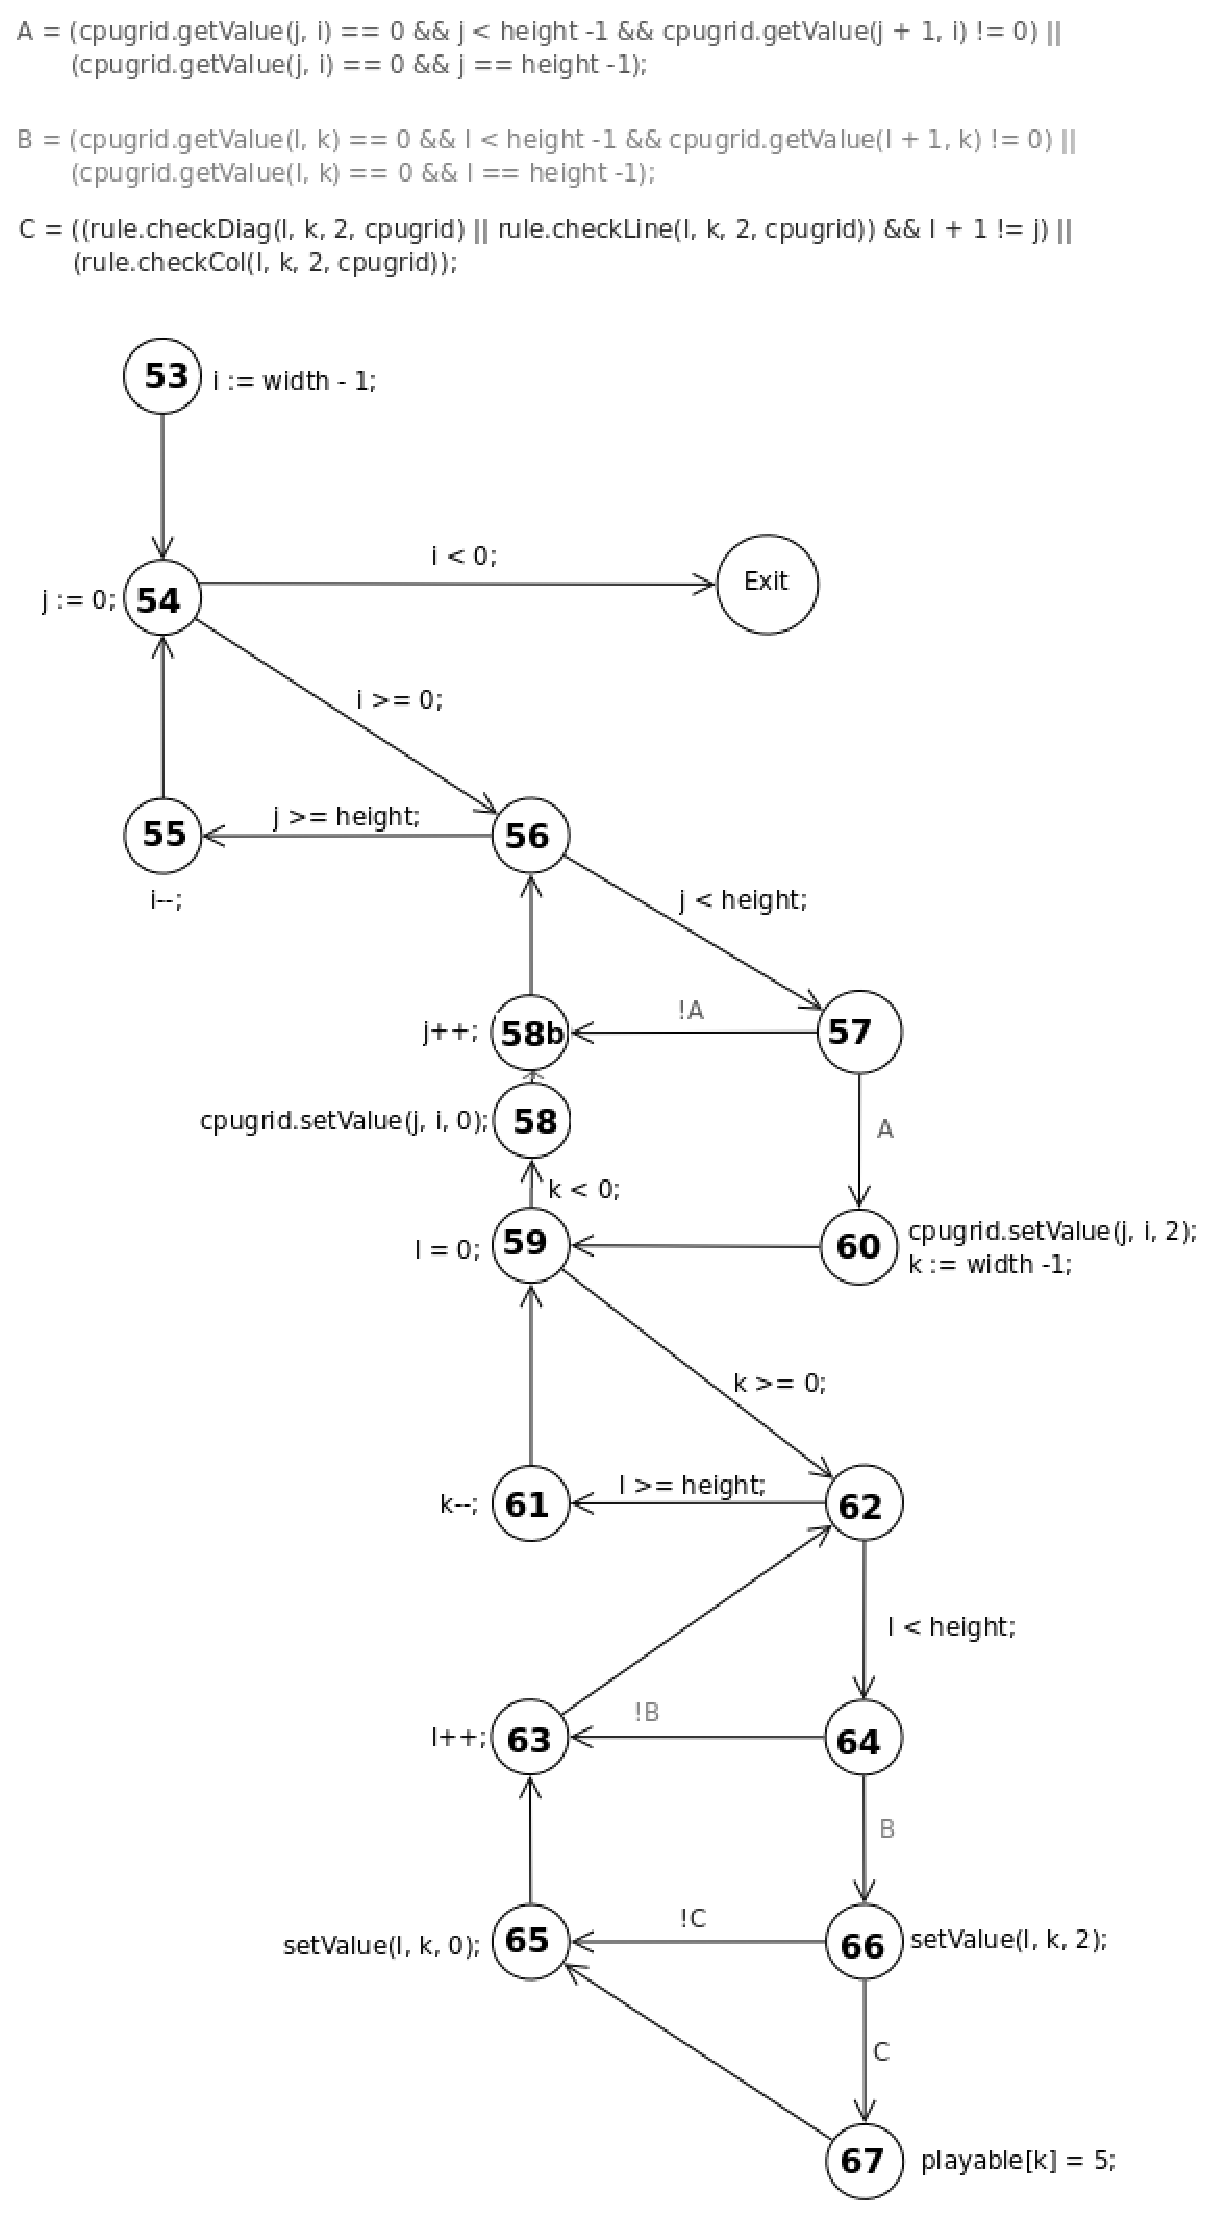
\includegraphics[scale=0.4]{strategy}
  \caption{Fonction figure}
\end{center}
\end{figure}